%%%%%%%%%%%%%%%%%%%%%%%%%%%%%%%%%%%%%%%%%
% University/School Laboratory Report
% LaTeX Template
% Version 3.1 (25/3/14)
%
% This template has been downloaded from:
% http://www.LaTeXTemplates.com
%
% Original author:
% Linux and Unix Users Group at Virginia Tech Wiki 
% (https://vtluug.org/wiki/Example_LaTeX_chem_lab_report)
%
% License:
% CC BY-NC-SA 3.0 (http://creativecommons.org/licenses/by-nc-sa/3.0/)
%
%%%%%%%%%%%%%%%%%%%%%%%%%%%%%%%%%%%%%%%%%

%----------------------------------------------------------------------------------------
%	PACKAGES AND DOCUMENT CONFIGURATIONS
%----------------------------------------------------------------------------------------

\documentclass{article}

\usepackage[version=3]{mhchem} % Package for chemical equation typesetting
\usepackage{siunitx} % Provides the \SI{}{} and \si{} command for typesetting SI units
\usepackage{graphicx} % Required for the inclusion of images
\usepackage{natbib} % Required to change bibliography style to APA
\usepackage{amsmath} % Required for some math elements 
\usepackage[a4paper,margin=0.5in]{geometry}
\setlength\parindent{0pt} % Removes all indentation from paragraphs

\renewcommand{\labelenumi}{\alph{enumi}.} % Make numbering in the enumerate environment by letter rather than number (e.g. section 6)

%\usepackage{times} % Uncomment to use the Times New Roman font

%----------------------------------------------------------------------------------------
%	DOCUMENT INFORMATION
%----------------------------------------------------------------------------------------

\title{Gate Detection} % Title

\author{Philipp \textsc{Duernay}} % Author name

\date{\today} % Date for the report

\begin{document}
\maketitle
% If you wish to include an abstract, uncomment the lines below
% \begin{abstract}
% Abstract text
% \end{abstract}

%----------------------------------------------------------------------------------------
%	SECTION 1
%----------------------------------------------------------------------------------------

\section{Summary}

\begin{itemize}
	\item Implementation of Yolo Object Detector \cite{Redmon1,Redmon2} in Python (Keras, tensorflow)
	\item Verification of implementation by training and testing on Pascal VOC dataset
	\item Training Yolo on generated gate dataset
	\item Evaluation of Yolo with respect to camera position
\end{itemize}


\section{Set Generation}

\begin{itemize}
	\item at most 1 gate per image
	\item gate taken from IROS 2017 (2.5m square gate)
	\item background pictures from Pascal VOC dataset
	\item camera positions 10000 randomly samples within the following parameters: $$ \Phi \in [-\frac{\pi}{2},\frac{\pi}{2}] \quad \Theta \in [-\frac{\pi}{2},\frac{\pi}{2}] \quad \Psi \in [-\frac{\pi}{2},\frac{\pi}{2}] \quad X = [-5, -15] \quad Y = [0.5,0.5]Z = [-0.5,0.5]$$ where $1 \rightarrow 0.85m$
	\item Image format: BGR,YUV (one set each)
\end{itemize}

\subsection{Training Parameters}
\begin{itemize}
	\item sample size = 60600, 60000 containing one gate, 600 containing no gate
	\item epochs=100 (early stop after ~20), batch size=8, training size = 90\%, validation size = 10\%
	\item solver: adam, $\alpha = 0.001$, $\beta_1 = 0.9$, $\beta_2 = 0.999$
\end{itemize}
\subsection{Test Set}
\begin{itemize}
	\item sample size = 1100, 1000 containing one gate, 100 containing no gate
\end{itemize}

\section{Results}
\begin{figure}[!htb]
	\centering
	\begin{minipage}{.5\textwidth}
		\centering
		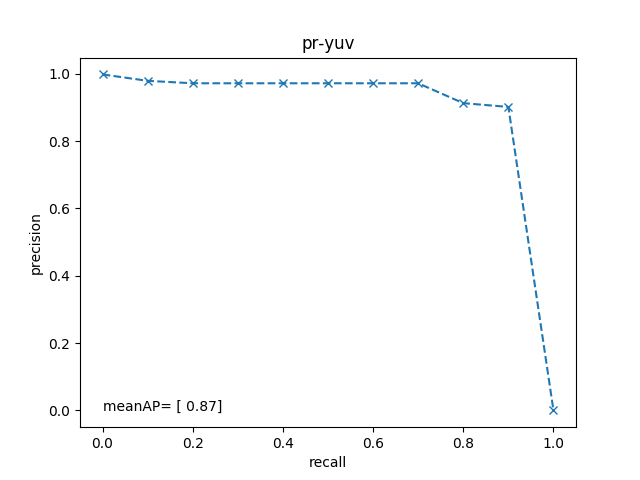
\includegraphics[width=0.9\textwidth]{yolo-gate-yuv-1000}
		\caption{Yolo on YUV-set at different confidence levels. Testset size =1000}
	\end{minipage}%
	\begin{minipage}{0.5\textwidth}
		\centering
		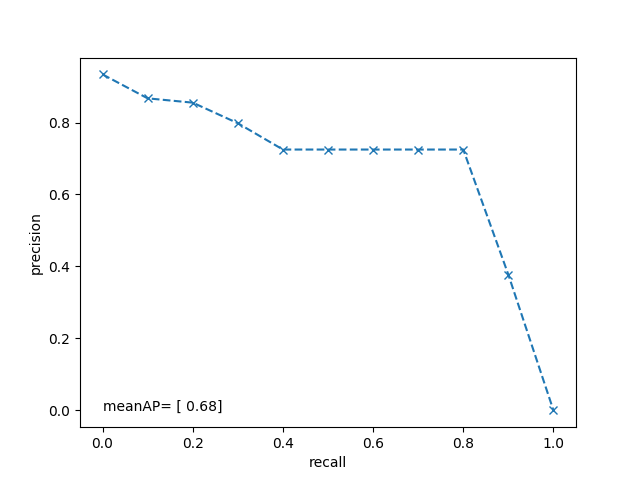
\includegraphics[width=0.9\textwidth]{yolo-gate-1000}
		\caption{Yolo on BGR-set at different confidence levels. Testset size =1000}
	\end{minipage}
\end{figure}
\begin{figure}[!htb]
	\centering
	\begin{minipage}{.5\textwidth}
		\centering
		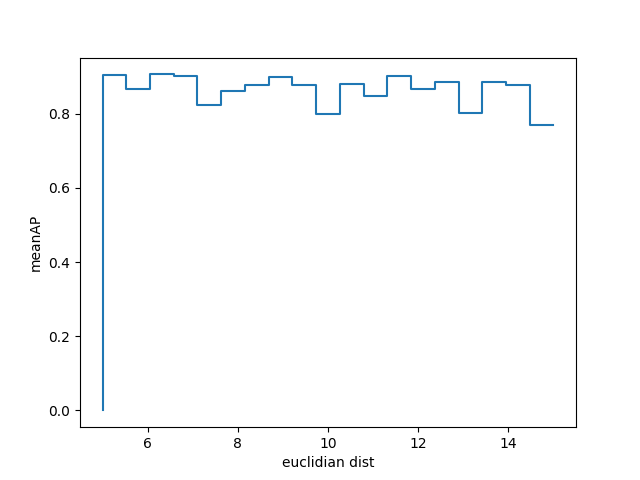
\includegraphics[width=0.9\textwidth]{meanAP-eucl}
		\caption{AP over Distance on YUV}
	\end{minipage}%
	\begin{minipage}{0.5\textwidth}
		\centering
		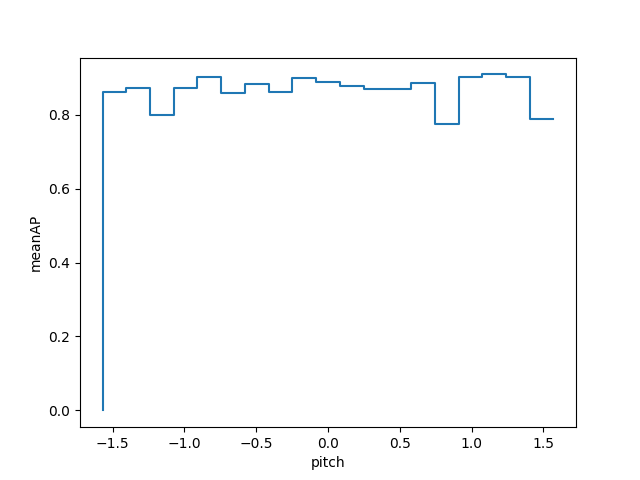
\includegraphics[width=0.9\textwidth]{meanAP-pitch}
		\caption{AP over Pitch angle on YUV}
	\end{minipage}
	\begin{minipage}{.5\textwidth}
		\centering
		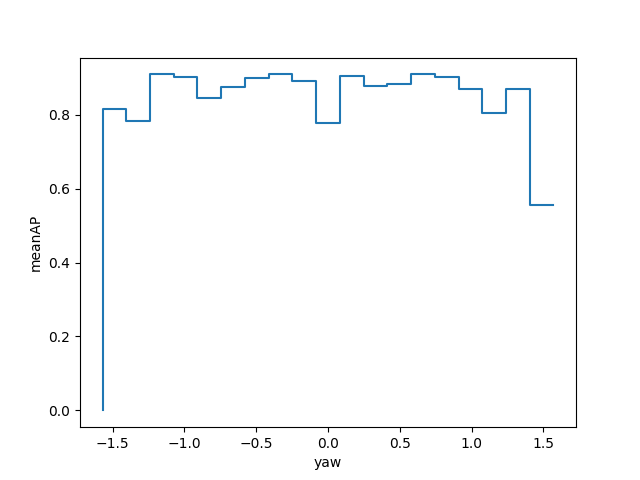
\includegraphics[width=0.9\textwidth]{meanAP-yaw}
		\caption{AP over Yaw angle on YUV }
	\end{minipage}%
	\begin{minipage}{0.5\textwidth}
		\centering
		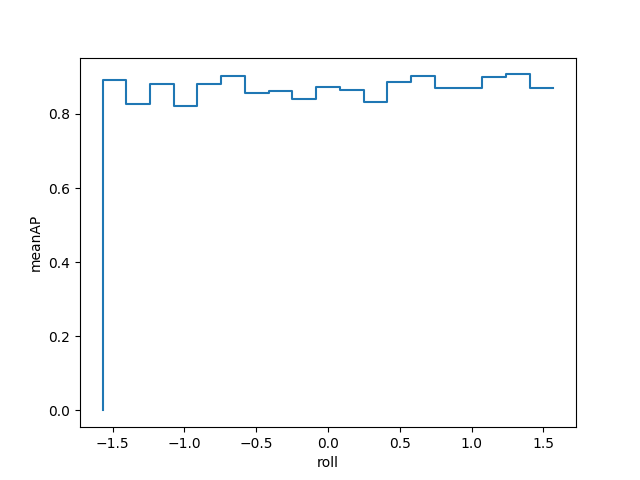
\includegraphics[width=0.9\textwidth]{meanAP-roll}
		\caption{AP over Roll angle on YUV}
	\end{minipage}
\end{figure}
\section{Conclusions}
\begin{itemize}
	\item Much better results with YUV format
	\item No real influence of angle/distance measurable
\end{itemize}
\section{Next Step}
\begin{itemize}
	\item Evaluate on cases where gate is close to border
	\item Try to break it
	\item compare to other models e.g. SSD
	\item Test how precise bounding boxes are
\end{itemize}

%----------------------------------------------------------------------------------------


%----------------------------------------------------------------------------------------
%	BIBLIOGRAPHY
%----------------------------------------------------------------------------------------

\bibliographystyle{abbrv}

\bibliography{bib}

%----------------------------------------------------------------------------------------


\end{document}